

%% AAPT Physics Olympiad F=ma Questions
%%----------------------------------------


%% PhysicsOlympiad 2015
%%----------------------------------------


%% PhysicsOlympiad 2000
%%----------------------------------------
\element{aapt}{ %% Olympiad-B2
\begin{question}{olympiad-2000-q11}
    Light with an angle of incidence of \ang{57} in air is completely polarized when it reflects off a sheet of plate glass.
    What is the index of refraction of the glass?
    \begin{multicols}{3}
    \begin{choices}
        \wrongchoice{0.649}
        \wrongchoice{1.19}
        \wrongchoice{1.41}
      \correctchoice{1.54}
        \wrongchoice{1.84}
    \end{choices}
    \end{multicols}
\end{question}
}

\element{aapt}{ %% Olympiad-B2
\begin{question}{olympiad-2000-q21}
    A converging lens has a focal length of \SI{10}{\centi\meter}.
    If an object is placed \SI{50}{\centi\meter} from the lens,
        what will be the magnitude of the magnification of the image?
    \begin{multicols}{3}
    \begin{choices}
        \wrongchoice{$\dfrac{1}{5}$}
      \correctchoice{$\dfrac{1}{4}$}
        \wrongchoice{$\dfrac{1}{2}$}
        \wrongchoice{2}
        \wrongchoice{5}
    \end{choices}
    \end{multicols}
\end{question}
}


%% PhysicsOlympiad 1998
%%----------------------------------------
\element{aapt}{ %% Olympiad-B2
\begin{question}{olympiad-1998-q24}
    An object is placed \SI{12}{\centi\meter} in front of a spherical mirror.
    The image is right side up and is two times bigger than the object.
    The image is:
    \begin{choices}
        \wrongchoice{\SI{6}{\centi\meter} in front of the mirror and real.}
        \wrongchoice{\SI{6}{\centi\meter} behind the mirror and virtual.}
        \wrongchoice{\SI{12}{\centi\meter} in front of the mirror and virtual.}
        \wrongchoice{\SI{24}{\centi\meter} in front of the mirror and virtual.}
      \correctchoice{\SI{24}{\centi\meter} behind the mirror and virtual.}
    \end{choices}
\end{question}
}


%% PhysicsOlympiad 1997
%%----------------------------------------
\element{aapt}{ %% Olympiad-B2
\begin{question}{olympiad-1997-q20}
    You are given two lenses,
        a converging lens with focal length \SI{+10}{\centi\meter} and a diverging lens with focal length \SI{-20}{\centi\meter}.
    Which of the following would produce a virtual image that is larger than the object?
    \begin{choices}
      \correctchoice{Placing the object \SI{5}{\centi\meter} from the converging lens.}
        \wrongchoice{Placing the object \SI{15}{\centi\meter} from the converging lens.}
        \wrongchoice{Placing the object \SI{25}{\centi\meter} from the converging lens.}
        \wrongchoice{Placing the object \SI{15}{\centi\meter} from the diverging lens.}
        \wrongchoice{Placing the object \SI{25}{\centi\meter} from the diverging lens.}
    \end{choices}
\end{question}
}


%% PhysicsOlympiad 1996
%%----------------------------------------
\element{aapt}{ %% Olympiad-B2
\begin{question}{olympiad-1996-q20}
    You are given two lenses, a converging lens with focal length \SI{+10}{\centi\meter} and a diverging lens with focal length \SI{-20}{\centi\meter}.
    Which of the following would produce a real image that is larger than the object?
    \begin{choices}
        \wrongchoice{Placing the object \SI{5}{\centi\meter} from the converging lens.}
      \correctchoice{Placing the object \SI{15}{\centi\meter} from the converging lens.}
        \wrongchoice{Placing the object \SI{25}{\centi\meter} from the converging lens.}
        \wrongchoice{Placing the object \SI{15}{\centi\meter} from the diverging lens.}
        \wrongchoice{Placing the object \SI{25}{\centi\meter} from the diverging lens.}
    \end{choices}
\end{question}
}

\element{aapt}{ %% Olympiad-B2
\begin{question}{olympiad-1996-q21}
    Two mirrors, labeled $LM$ for left mirror and $RM$ for right mirror in the accompanying figure,
        are parallel to each other and \SI{3.0}{\meter} apart. 
    \begin{center}
    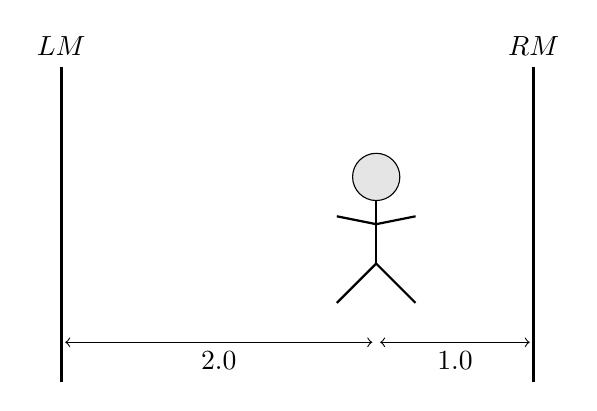
\begin{tikzpicture}
        %% Left and right mirror
        \draw[very thick] (-4,-1) -- (-4,3) node[anchor=south] {$LM$};
        \draw[very thick] (+2,-1) -- (+2,3) node[anchor=south] {$RM$};
        %% Arrows
        \draw[<->] (-3.95,-0.5) -- (-0.05,-0.5) node[pos=0.5,anchor=north] {\SI{2.0}{\meter}};
        \draw[<->] (+1.95,-0.5) -- (+0.05,-0.5) node[pos=0.5,anchor=north] {\SI{1.0}{\meter}};
        %%% Man
        \begin{scope}[anchor=south,scale=2.0]
            \draw[thick] (0,0.25) -- (0,0.75);
            %% Legs
            \draw[thick] (0,0.25) -- (-0.25,0);
            \draw[thick] (0,0.25) -- (+0.25,0);
            %% Arms
            \draw[thick] (0,0.50) -- (-0.25,0.55);
            \draw[thick] (0,0.50) -- (+0.25,0.55);
            %% Head
            \draw[fill=white!90!black] (0,0.80) circle (0.15cm);
        \end{scope}
    \end{tikzpicture}
    \end{center}
    A person standing \SI{1.0}{\meter} from the right mirror ($RM$) looks into this mirror and sees a series of images. 
    How far from the person is the second closest image seen in the right mirror ($RM$)?
    \begin{multicols}{3}
    \begin{choices}
        \wrongchoice{\SI{2.0}{\meter}}
        \wrongchoice{\SI{4.0}{\meter}}
      \correctchoice{\SI{6.0}{\meter}}
        \wrongchoice{\SI{8.0}{\meter}}
        \wrongchoice{\SI{10.0}{\meter}}
    \end{choices}
    \end{multicols}
\end{question}
}


%% PhysicsOlympiad 1995
%%----------------------------------------
\element{aapt}{ %% Olympiad-B2
\begin{question}{olympiad-1995-q21}
    You are given two lenses,
        a converging lens with focal length \SI{+10}{\centi\meter} and a diverging lens with focal length \SI{-20}{\centi\meter}.
    Which of the following would produce a virtual image that is larger than the object?
    \begin{choices}
      \correctchoice{Placing the object \SI{5}{\centi\meter} from the converging lens.}
        \wrongchoice{Placing the object \SI{15}{\centi\meter} from the converging lens.}
        \wrongchoice{Placing the object \SI{25}{\centi\meter} from the converging lens.}
        \wrongchoice{Placing the object \SI{15}{\centi\meter} from the diverging lens.}
        \wrongchoice{Placing the object \SI{25}{\centi\meter} from the diverging lens.}
    \end{choices}
\end{question}
}


%% PhysicsOlympiad 1994
%%----------------------------------------
\element{aapt}{ %% Olympiad-B2
\begin{question}{olympiad-1994-q21}
    You are given two lenses,
        a converging lens with focal length \SI{+10}{\centi\meter} and a diverging lens with focal length \SI{-20}{\centi\meter}.
    Which of the following would produce a real image that is smaller than the object?
    \begin{choices}
        \wrongchoice{Placing the object \SI{5}{\centi\meter} from the converging lens.}
        \wrongchoice{Placing the object \SI{15}{\centi\meter} from the converging lens.}
      \correctchoice{Placing the object \SI{25}{\centi\meter} from the converging lens.}
        \wrongchoice{Placing the object \SI{15}{\centi\meter} from the diverging lens.}
        \wrongchoice{Placing the object \SI{25}{\centi\meter} from the diverging lens.}
    \end{choices}
\end{question}
}



\endinput


